

\chapter{Despliegue en contenedores}
Una vez desarrollados los microservicios y su monitorización, es necesario ponerlos en producción, y una de las decisiones importantes es dónde queremos que corran, si en máquinas físicas, máquinas virtuales o en contenedores (en nuestro caso, se descarta la opción de implementarlo en \textit{Cloud}). La decisión tomada es que todo corra sobre contenedores en una plataforma \textit{\textbf{OCP}} \textit{Openshift Container Platform}, los motivos de esta decisión son los siguientes: 

\begin{itemize}
	\item \textit{\textbf{Stateless}}: Todos los servicios implementados no necesitan estado (los datos necesarios se almacenan en el bus). Lo que lo hace un caso de uso ideal para su ejecución en contenedores. 
	\item \textbf{Agilidad de despliegue}: El proceso de creación y destrucción de un contenedor es inmediato, lo que no da mucha flexibilidad a la hora desplegar nuevos contenedores.
	
	\item \textbf{Serivicios Autocontenidos}: Los contenedores pueden ejecutarse en multitud de plataformas lo que nos permite tener aplicaciones inmutables y autocontenidas que podemos mover entre plataformas y entornos. Este punto y el anterior serán de mucha utilidad a la hora de implementar la integración y el despliegue continuo.
	
	\item  \textbf{Alta disponibilidad}: Al tener un clúster de \textit{Openshift} con múltiples nodos, en el caso que se produjera un fallo en un nodo que provocara la caída de un contenedor, este se levantaría automáticamente en otro nodo. 
	
\end{itemize} 

A la largo del apartado nos referiremos a los siguientes conceptos propios de \textit{Openshift} (muchos de ellos heredados en \textit{Kubernetes}):

\begin{itemize}
\item  \textit{\textbf{Pod}}: Un pod es la unidad mínima en \textit{OCP}. Puede estar formado por uno o varios contenedores (\textit{Docker}), pero todos ellos correrán en una única máquina y tendrán una única dirección IP.

\item  \textit{\textbf{Despliegue}}: Un despliegue (\textit{Deployment}) podemos decir, de una manera muy simplificada, que gestiona el número de réplicas de un \textit{pod}. 

\item  \textbf{Configuración de despliegue}: La configuración de despliegue (\textit{Deployment Config}) dota a los despliegues de un ciclo de vida proporcionando versiones de los mismo, disparadores para crear nuevos despliegues de manera automática y estrategias para realizar transiciones entre diferentes versiones de despliegues sin pérdida de servicio. 

\item  \textbf{Servicio}: Un servicio expone un número determinado de Pods para que sean accesibles desde otros elementos de la plataforma. 

\item  \textbf{\textit{ConfigMap}}: Se trata de un mecanismo de \textit{OCP} para almacenar elementos de configuración mediante un mecanismo de clave-valor. Es posible almacenar tanto ficheros como valores simples.


\end{itemize}

\begin{figure}[!ht]
	\centering
	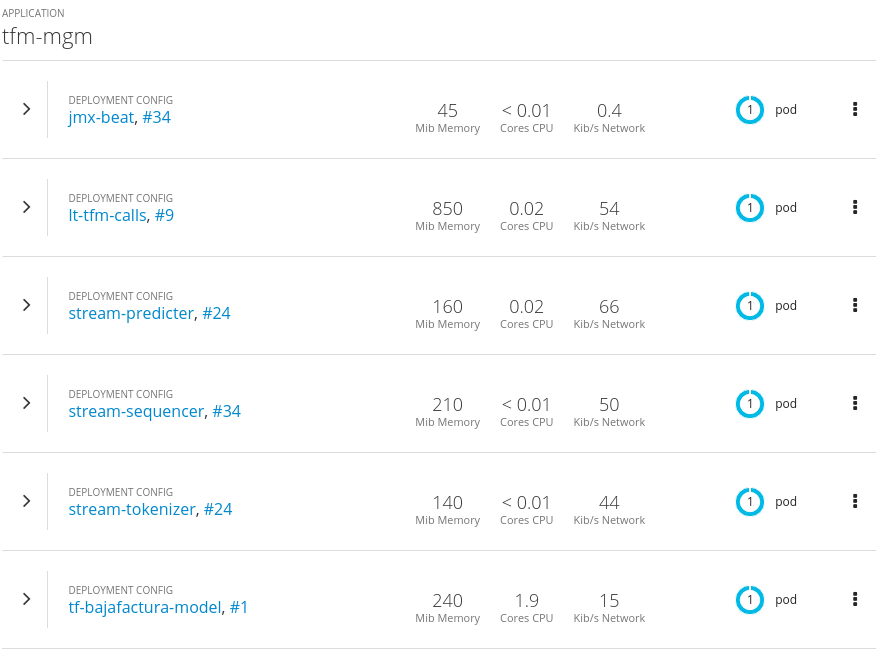
\includegraphics[width=1\textwidth]{images/cont/overview}
	\caption{configuración de despliegue y recursos usados en OCP}
	\label{fig:ocp-overview}
\end{figure}

En la figura \ref{fig:ocp-overview} podemos ver las diferentes configuraciones de despliegue con los \textit{pods} que tienen levantados cada uno y los recursos de memoria, cpu y red que consumen cada uno. 
 
A continuación veremos un resumen de los servicios, despliegues y configuraciones desplegadas en Openshift para cada tipo de microservicio y monitorización. En el apéndice \cite{apendi:contenedores} podemos encontrar todo el código de despliegue en Openshift, que nos permitiría desplegar todo nuestro entorno en otro clúster en cuestión de minutos. 


\section{Servicios \textit{Kafka Streams}}

Para desplegar los servicios de \textit{Kafka Streams} en \textit{OCP} es necesario desplegar una  configuración de despliegue por microservicio, un servicio para exponer las métricas y disponer en un \textit{configmap} de las opciones necesarias para su ejecución. 

En este apartado únicamente presentaremos a modo de ejemplo la configuración de despliegue y el servicio  del microservicio \textit{Predicter} explicando las características más relevantes del mismo. Tanto el \textit{configmap} con todos los ficheros como el resto de despliegues pueden consultarse en el apéndice \cite{apendi:contenedores}. 

La configuración de despliegue de \textit{Predicter} es la siguiente: 

\begin{minted}[
	gobble=0,
	frame=single,
	linenos
	]{yaml}

apiVersion: apps.openshift.io/v1
kind: DeploymentConfig
metadata:
  labels:
    app: tfm-mgm
    project: topic-model
    service: stream-predicter
  name: stream-predicter
  namespace: nbia-prod
spec:
  replicas: 1
  revisionHistoryLimit: 10
  selector:
    deploymentconfig: stream-predicter
  strategy:
    activeDeadlineSeconds: 21600
    recreateParams:
      timeoutSeconds: 600
    resources: {}
    type: Recreate
  template:
    metadata:
      creationTimestamp: null
      labels:
        app: tfm-mgm
        deploymentconfig: stream-predicter
        project: topic-model
        service: calls-predicter
    spec:
      containers:
        - env:
            - name: JAVA_MAIN_CLASS
              value: com.telefonica.topicmodel.PredicterLauncher
          image: >-
            docker-registry.default.svc:5000/nbia-prod/
            topic-model-streaming:latest
          imagePullPolicy: Always
          name: stream-predicter
          ports:
            - containerPort: 8778
              protocol: TCP
          resources:
            limits:
              cpu: '1'
              memory: 512Mi
            requests:
              cpu: 200m
              memory: 256Mi
          terminationMessagePath: /dev/termination-log
          terminationMessagePolicy: File
          volumeMounts:
            - mountPath: /opt/jolokia/etc/jolokia.properties
              name: calls-config
              subPath: jolokia.properties
            - mountPath: /deployments/application.json
              name: calls-config
              subPath: topic-model-streaming.json
      dnsPolicy: ClusterFirst
      restartPolicy: Always
      schedulerName: default-scheduler
      terminationGracePeriodSeconds: 30
      volumes:
        - configMap:
            defaultMode: 420
            name: calls-config
          name: calls-config
  test: false
  triggers:
    - imageChangeParams:
        automatic: true
        containerNames:
          - stream-predicter
        from:
          kind: ImageStreamTag
          name: 'topic-model-streaming:latest'
          namespace: nbia-prod
      type: ImageChange
    - type: ConfigChange

\end{minted}

Del despliegue anteriormente expuesto podemos destacar las siguientes características: 

\begin{itemize}
	\item \textbf{labels} (línea 4):  Nos ayudan a identificar el despliegue, el proyecto y la aplicación. Todos los despliegues relacionados con el TFM que se presentan en este documento tendrán el indicador \textit{tfm-mgm}. 

	\item \textbf{replicas} (línea 11): Indica el número de réplicas de cada \textit{pod} que pueden correr al mismo tiempo. En este caso lo establecemos a uno, pero podría escalar horizontalmente incluso hacerlo de manera automática por uso de CPU o memoria mediante un \textit{Horizontal Pod Autoscaler}. 



	\item \textbf{strategy} (línea 15): Establecemos la estrategia con la que se implantará una nueva versión del \textit{deployment}, en este caso utilizamos una estrategia \textit{Recreate} que detiene todos los servicios de un \textit{deployment} anterior antes de iniciar uno nuevo. Debido a que el bus tiene capacidad de retención de los eventos, esto no implicará una interrupción en el servicio, si no un ligero retraso en los eventos que se ingesten durante el despliegue.

	\item \textbf{Container} (línea 30): Aquí encontramos toda la información del contenedor que se desplegará. Destacamos: 
		\begin{itemize}
			\item \textbf{env} (línea 31): Variables globales del \textit{deploynment}, en este caso la clase Java  principal que se lanzará al ejecutar el contenedor. 
			\item \textbf{image} (línea 34): Contiene la referencia a la imagen del contenedor que queremos desplegar. Se trata de una imagen de Java con nuestro código que se encuentra almacenada en el repositorio de la plataforma. El parámetro \textit{imagePullPolicy} indica en qué circunstancias se descargará la imagen del repositorio (en este caso lo hará siempre, exista o no en el nodo en el que se despliega el \textit{Pod}).
			\item \textbf{Ports} (línea 34): Indica los puertos que expondrá el contenedor, en este caso se expondrá únicamente el puerto 8778 que es el puerto por defecto del \textit{endpoint} de \textit{Jolokia}.
			\item \textbf{Resources} (línea 42): Contiene los recursos de CPU y memoria que solicitará el \textit{Pod}  al arrancar y a los que estara limitados. 
			\item \textbf{VolumeMounts} (línea 51): Indica los volúmenes que montará el contenedor, en este caso son todos procedentes de un \textit{configmap} y contienen los ficheros de configuración de \textit{jolokia} y de la aplicación.
		\end{itemize}
	\item  \textbf{volumes} (línea 62): Contiene los volúmenes que se utilizaran en los contenedores en el apartado \textit{VolumeMounts}. En este caso unicamente contiene un \textit{configmap}. 
	\item \textbf{triggers} (línea 68): Define los disparadores que provocarán que se realice un nuevo \textit{deployment}, en este caso la modificación de la imagen o la modificación de la configuración de despliegue.

\end{itemize}


El servicio de \textit{Predicter} es el siguiente: 

\begin{minted}[
	gobble=0,
	frame=single,
	linenos
	]{yaml}

apiVersion: v1
kind: Service
metadata:
  labels:
    app: tfm-mgm
  name: stream-predicter
  namespace: nbia-prod
spec:
  ports:
    - name: 8778-tcp
      port: 8778
      protocol: TCP
      targetPort: 8778
  selector:
    deploymentconfig: stream-predicter
  sessionAffinity: None
  type: ClusterIP

\end{minted}

Aparte de las etiquetas que tienen las misma utilidad que la configuración de despliegue vista anteriormente, cabe destacar los siguientes parámetros: 

\begin{itemize}
	\item \textbf{name} (línea 6): El nombre del servicio que usaremos para llamarlo dentro de la plataforma. 
	 \item \textbf{ports} (línea 9): El puerto que expondrá el servicio y al puerto de los \textit{pods} que atacará. 
	 \item \textbf{selector} (línea 14): Los \textit{pods} a los que atacará el servicio. En este caso los \textit{pods} pertenecientes al configuración de despliegue \textit{stream-predicter}. 
	 
	 \item \textbf{sessionAffinity} (línea 16): Si quisieramos establecer alguna afinidad, por ejemplo a nivel de \textit{IP}, para que un mismo origen ataque siempre a un mismo \textit{Pod}. Hay que recordar que los servicios en \textit{Openshift} (y \textit{Kubernetes}) actúan como un balanceador entre los \textit{pods}.
\end{itemize}




\section{Servicios \textit{Tensorflow Serving}}

En el caso del servicio de Tensorflow Serving, mostraremos únicamente la configuración de despliegue, aunque también consta de un servicio para que podamos realizar llamadas \textit{HTTP} sobre el mismo desde la plataforma de \textit{Openshift}. En el caso de que se quisiera acceder al servicio desde fuera de la plataforma será necesario recurrir las \textit{Routes} de Openshift.

La configuración de despliegue de \textit{tf-BajaFactura} es la siguiente:

 
\begin{minted}[
	gobble=0,
	frame=single,
	linenos
	]{yaml}
apiVersion: apps.openshift.io/v1
kind: DeploymentConfig
metadata:
  labels:
    app: tfm-mgm
    appName: tf-bajafactura-model
    appTypes: tensorflow-serving-s2i
    appid: tf-serving-tf-bajafactura-model
  name: tf-bajafactura-model
  namespace: nbia-prod
spec:
  replicas: 1
  revisionHistoryLimit: 10
  selector:
    deploymentconfig: tf-bajafactura-model
  strategy:
    activeDeadlineSeconds: 21600
    rollingParams:
      intervalSeconds: 1
      maxSurge: 25%
      maxUnavailable: 25%
      timeoutSeconds: 600
      updatePeriodSeconds: 1
    type: Rolling
  template:
    metadata:
      labels:
        app: tfm-mgm
        appName: tf-bajafactura-model
        appTypes: tensorflow-serving-s2i
        appid: tf-serving-tf-bajafactura-model
        deploymentconfig: tf-bajafactura-model
    spec:
      containers:
        - env:
            - name: PORT
              value: '8501'
            - name: MODEL_NAME
              value: bajafactura
            - name: RUN_OPTIONS
          image: >-
            docker-registry.default.svc:5000/nbia-prod/
            tf-bajafactura-model:latest
          imagePullPolicy: Always
          livenessProbe:
            failureThreshold: 10
            httpGet:
              path: /v1/models/bajafactura
              port: 8501
              scheme: HTTP
            initialDelaySeconds: 20
            periodSeconds: 30
            successThreshold: 1
            timeoutSeconds: 5
          name: tf-bajafactura-model
          ports:
            - containerPort: 8501
              protocol: TCP
          readinessProbe:
            failureThreshold: 1
            httpGet:
              path: /v1/models/bajafactura
              port: 8501
              scheme: HTTP
            initialDelaySeconds: 20
            periodSeconds: 10
            successThreshold: 1
            timeoutSeconds: 5
          resources:
            limits:
              cpu: '2'
              memory: 2Gi
            requests:
              cpu: '1'
              memory: 1Gi
          terminationMessagePath: /dev/termination-log
          terminationMessagePolicy: File
      dnsPolicy: ClusterFirst
      restartPolicy: Always
      schedulerName: default-scheduler
      terminationGracePeriodSeconds: 30
  test: false
  triggers:
    - imageChangeParams:
        automatic: true
        containerNames:
          - tf-bajafactura-model
        from:
          kind: ImageStreamTag
          name: 'tf-bajafactura-model:latest'
          namespace: nbia-prod
      type: ImageChange
    - type: ConfigChange


\end{minted}

En este caso solo comentaremos los parámetros que varían con respecto al despliegue de los servicios \textit{Kafka Streams}: 
\begin{itemize}
	\item \textbf{strategy} (línea 16): En este caso la estrategia en el caso de que exista un nuevo despliegue se denomina \textit{Rolling}. Esto implica, de forma muy resumida, que el nuevo \textit{deployment} se hará de manera paulatina, no eliminando los \textit{deployment} anteriores hasta que no se hayan realizado los nuevos. Esto garantiza que no exista una pérdida de servicio en los nuevos despliegues.  
	\item \textbf{image} (línea 41): La imagen usada en este caso es la imagen de \textit{docker} de TensorFlow Serving con nuestro modelo cargado, esta imagen  se encuentra almacenada en el repositorio de la plataforma.
	\item \textbf{livenessProbe} (línea 45): Comprueba que el contenedor sigue con vida, de no ser así durante el número de intentos establecido se reiniciará el contenedor. En este caso la comprobación es una petición \textit{HTTP} al \textit{endpoint} de estado del modelo.
	 \item \textbf{readinessProbe} (línea 59): Antes de enviar tráfico a un \textit{pod}, este debe estar en estado \textit{ready}. Con este parámetro establecemos que el \textit{pod} no se encuentre \textit{ready} hasta que no se haya verificado el \textit{endpoint} de estado del modelo.
\end{itemize}

Aunque existen otros parámetros que varían como las variables de entornos o los recursos definidos el funcionamiento es igual a la configuración de despliegue definida anteriormente.


\section{Monitorización}

Los despliegues vistos hasta ahora nos permiten tener funcionando nuestro sistema, sin embargo, no debemos olvidarnos de la monitorización necesaria, que ya describimos en el capítulo \ref{chapter:prod}, para verificar el correcto funcionamiento del mismo. 

Dentro de Openshift la monitorización esta formada por dos despliegues diferentes:

\begin{itemize}
\item \textbf{Logstash}: Podemos identificarlo en la figura \ref{fig:ocp-overview} con el nombre \textbf{lt-tfm-calls} y será el encargado de llevar a la capa de servicio no solo la monitorización de todo el sistema, si no también los datos de clasificación de llamadas y  de realizar las transformaciones necesarias. 

\item \textbf{Metricbeat}: Podemos identificarlo en la figura \ref{fig:ocp-overview} con el nombre \textbf{jmx-beat} y será el encargado de extraer las métricas de Jolokia de los servicios de \textit{Kafka Streams}. 
\end{itemize}

A continuación veremos la configuración de ambos despliegues.

\subsection{Logstash}
Al igual que en los casos anteriores, vemos unicamente la configuración del despliegue, pudiendo encontrar el resto de recursos en el anexo \ref{anexo}. 

La configuración de despliegue es la siguiente:

\begin{minted}[
 	gobble=0,
 	frame=single,
 	linenos]{yaml}
apiVersion: apps.openshift.io/v1
kind: DeploymentConfig
metadata:
  labels:
    app: tfm-mgm
    service: lt-tfm-calls
    version: '1.0'
  name: lt-tfm-calls
  namespace: nbia-prod
spec:
  replicas: 1
  revisionHistoryLimit: 10
  selector:
    deploymentconfig: lt-tfm-calls
  strategy:
    activeDeadlineSeconds: 21600
    resources: {}
    rollingParams:
      intervalSeconds: 1
      maxSurge: 25%
      maxUnavailable: 25%
      timeoutSeconds: 600
      updatePeriodSeconds: 1
    type: Rolling
  template:
    metadata:
      labels:
        app: tfm-mgm
        deploymentconfig: lt-tfm-calls
        service: lt-tfm-calls
        version: '1.0'
    spec:
      containers:
        - env:
            - name: PIPELINE
              value: tfm-calls
            - name: LS_JAVA_OPTS
              value: '-Xmx2g'
            - name: USER_LOGSTASH
              valueFrom:
                secretKeyRef:
                  key: username
                  name: logstash-internal-user
            - name: PASS_LOGSTASH
              valueFrom:
                secretKeyRef:
                  key: password
                  name: logstash-internal-user
          image: 'docker-registry.default.svc:5000/openshift/logstash:7.4.2'
          imagePullPolicy: IfNotPresent
          livenessProbe:
            failureThreshold: 10
            httpGet:
              path: /
              port: 9600
              scheme: HTTP
            initialDelaySeconds: 300
            periodSeconds: 30
            successThreshold: 1
            timeoutSeconds: 5
          name: lt-tfm-calls
          ports:
            - containerPort: 5010
              protocol: TCP
            - containerPort: 9600
              protocol: TCP
          readinessProbe:
            failureThreshold: 1
            httpGet:
              path: /
              port: 9600
              scheme: HTTP
            initialDelaySeconds: 120
            periodSeconds: 10
            successThreshold: 1
            timeoutSeconds: 5
          resources:
            limits:
              cpu: '1'
              memory: 2200Mi
            requests:
              cpu: 500m
              memory: 2Gi
          terminationMessagePath: /dev/termination-log
          terminationMessagePolicy: File
          volumeMounts:
            - mountPath: /usr/share/logstash/config/logstash.yml
              name: calls-config
              subPath: logstash.yml
      dnsPolicy: ClusterFirst
      restartPolicy: Always
      schedulerName: default-scheduler
      terminationGracePeriodSeconds: 30
      volumes:
        - configMap:
            defaultMode: 420
            name: calls-config
          name: calls-config
  test: false
  triggers:
    - type: ConfigChange
 
\end{minted}

 Algunas características que podemos observar diferentes a las vistas actualmente son: 
 
 \begin{itemize}
 \item \textit{\textbf{Secrets}} (líneas 40 y 45): En este despliegue vemos que las variables globales para la autenticación se cargan de un recurso de \textit{OCP} denominado \textit{Secret}, utilizado para almacenar información sensible.
 \item  \textit{\textbf{image}} (línea 49): En este caso la imagen no contiene ningún código propio como en resto de despliegues vistos anteriormente. Se trata de la imagen oficial de \textit{Elastic}. El código a ejecutar (\textit{pipeline}) se almacena de forma centralizada en \textit{Elasticsearch} y utilizamos la variable de entorno \textit{PIPELINE} y los ficheros de configuración (\textit{configmaps}) para acceder a la información. 
 \item \textit{\textbf{resources}} (línea 77): En este caso vemos que los recursos solicitados son mayores que en el resto de despliegues. Esto se debe a que el \textit{Heap} que tiene configurado la imagen de \textit{Logstash} por defecto es mayor, podría modificarse para optimizar el uso de recursos, pero no hemos tenido esa necesidad.
 \end{itemize}



\subsection{Metricbeat}

El último despliegue que nos queda por ver, es probablemente el más simple, el de \textit{Metricbeat}, el agente encargado de extraer las métricas de \textit{Jolokia} de los servicios de  \textit{Kafka Streams}. Este despliegue no tiene asociado ningún servicio, ya que no será llamado por otros componentes. 

La configuración de despliegue de \textit{Metricbeat} es la siguiente: 

\begin{minted}[
 	gobble=0,
 	frame=single,
 	linenos]{yaml}
apiVersion: apps.openshift.io/v1
kind: DeploymentConfig
metadata:
  labels:
    app: tfm-mgm
    deploymentconfig: jmx-beat
    service: jmx-beat
  name: jmx-beat
  namespace: nbia-prod
spec:
  replicas: 1
  selector:
    deploymentconfig: jmx-beat
  strategy:
    activeDeadlineSeconds: 21600
    resources: {}
    rollingParams:
      intervalSeconds: 1
      maxSurge: 25%
      maxUnavailable: 25%
      timeoutSeconds: 600
      updatePeriodSeconds: 1
    type: Rolling
  template:
    metadata:
      labels:
        app: tfm-mgm
        deploymentconfig: jmx-beat
        project: tfmmgm
        service: jmx-beat
    spec:
      containers:
        - env:
            - name: ELASTICSEARCH_USERNAME
              valueFrom:
                secretKeyRef:
                  key: username
                  name: logstash-internal-user
            - name: ELASTICSEARCH_PASSWORD
              valueFrom:
                secretKeyRef:
                  key: password
                  name: logstash-internal-user
          image: >-
            docker-registry.default.svc:5000/nbia-prod/metricbeat:7.4.2
          imagePullPolicy: Always
          name: jmx-beat
          resources:
            limits:
              cpu: '1'
              memory: 512Mi
          terminationMessagePath: /dev/termination-log
          terminationMessagePolicy: File
          volumeMounts:
            - mountPath: /usr/share/metricbeat/metricbeat.yml
              name: calls-config
              subPath: metricbeat.yml
            - mountPath: /usr/share/metricbeat/modules.d/jolokia.yml
              name: calls-config
              subPath: jolokia.yml
      dnsPolicy: ClusterFirst
      restartPolicy: Always
      schedulerName: default-scheduler
      terminationGracePeriodSeconds: 30
      volumes:
        - configMap:
            defaultMode: 292
            name: calls-config
          name: calls-config
  test: false
  triggers:
    - type: ConfigChange
    - imageChangeParams:
        automatic: true
        containerNames:
          - jmx-beat
        from:
          kind: ImageStreamTag
          name: 'metricbeat:7.4.2'
          namespace: nbia-prod
      type: ImageChange
\end{minted}

Todos los parámetros vistos en este despliegue deberían resultarnos ya familiares. La imagen de \textit{docker} usada en este caso también se trata de la imagen oficial desarrollada por \textit{Elastic}.


\section{S2I}
\label{section:cont:s2i}
Los despliegues en \textit{OCP} descritos a lo largo de este capítulo podrían clasificarse en dos: Aquellos que son imágenes oficiales con alguna configuración propia y aquellos que contienen código fuente o binarios propios. En el primer grupo se encuentra el agente \textit{Metricbeat} y \textit{Logstash} (aunque ejecuta código propio no está almacenado en la imagen), mientras que al segundo grupo pertenecen los microservicios de \textit{Kafka Streams} y el modelo de \textit{Tensorflow Serving}. A partir de ahora, nos centraremos en este segundo grupo.


\begin{figure}[!ht]
	\centering
	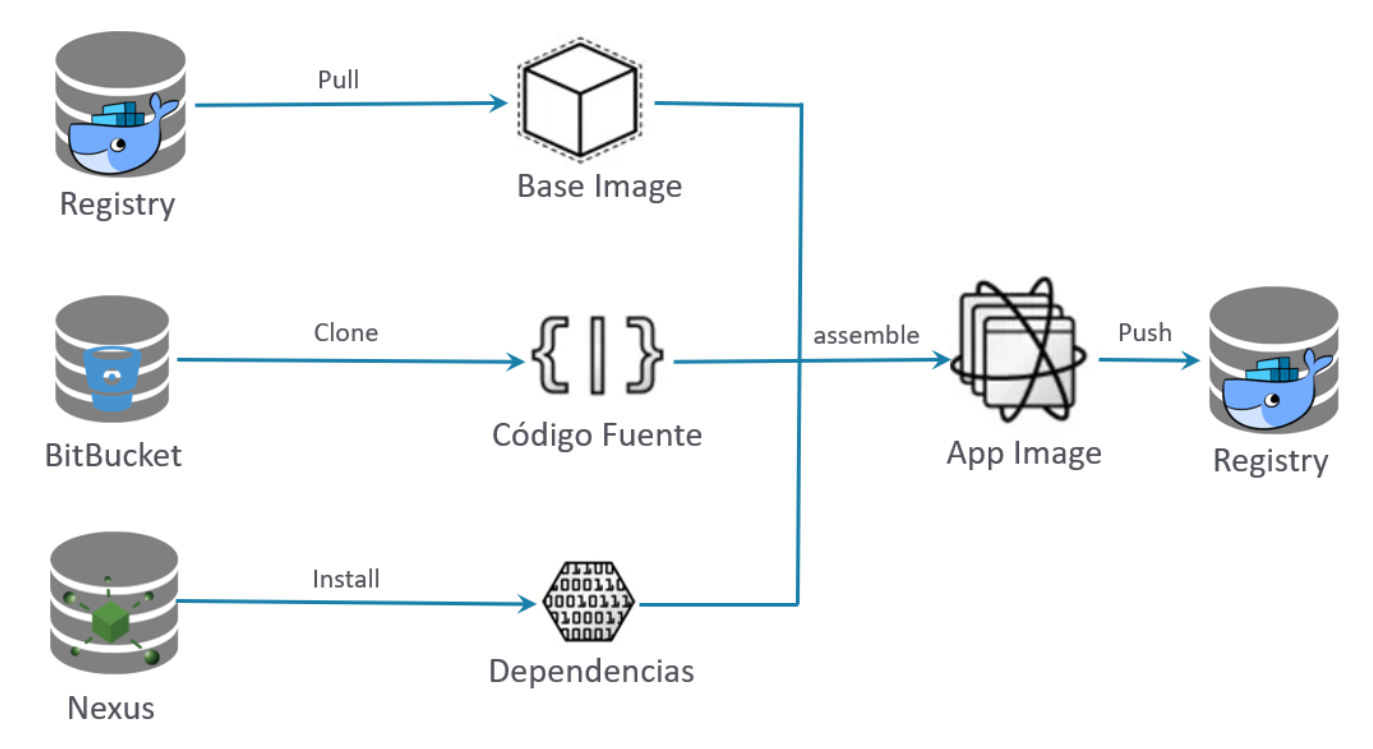
\includegraphics[width=1\textwidth]{images/cont/s2i}
	\caption{S2I en Openshift}
	\label{fig:ocp-s2i}
\end{figure}

La opción más simple para tener una imagen con nuestro código sería generarlas de forma individual y subirlas al repositorio de imágenes de la plataforma, sin embargo esta tarea se volvería algo tediosa conforme el número de servicios crezca, además presentaría dificultades en su mantenimiento y en su integración (como veremos más adelante) con flujos de integración y despliegue continuos. Es por eso que utilizaremos una característica de \textit{OCP} denominada \textit{S2I} (\textit{Sorce to Image}), que nos permitirá a partir de una imagen base (a partir de ahora imagen S2I) generar una nueva imagen personalizada con nuestra aplicación. En la figura \ref{fig:ocp-s2i}.

El proceso de crear la imagen de nuestra aplicación a partir de una imagen S2I y nuestro código o binarios se denomina \textit{Build} y al igual que con la configuración de despliegue para los despliegues \textit{Openshift}, nos proporciona una configuración de \textit{Build} para controlar las versiones y los cambios que se realizan en un mismo tipo de \textit{Build}. A continuación veremos como hemos abordado los casos de \textit{Kafka Streams} y \textit{Tensorflow Serving}.


\subsection{\textit{Kafka Streams}}

En este caso tenemos dos opciones a la hora de crear nuestra imagen de aplicación mediante S2I, partir del código fuente o partir de un binario (un jar generado a partir del código fuente). Hemos optado por esta segunda opción para dejar la compilación y tests fuera de la plataforma \textit{OCP}. 

La imagen \textit{S2I} utilizada es la imagen oficial proporcionada por RedHat para Java. Y a continuación podemos ver como quedaría nuestra configuración de \textit{Build}:

\begin{minted}[
 	gobble=0,
 	frame=single,
 	linenos]{yaml}
apiVersion: build.openshift.io/v1
kind: BuildConfig
metadata:
  labels:
    app: tfm-mgm
  name: topic-model-streaming
  namespace: nbia-prod
spec:
  failedBuildsHistoryLimit: 5
  output:
    to:
      kind: ImageStreamTag
      name: 'topic-model-streaming:latest'
  runPolicy: Serial
  source:
    binary: {}
    type: Binary
  strategy:
    sourceStrategy:
      from:
        kind: ImageStreamTag
        name: 'redhat-openjdk18-openshift:1.4'
        namespace: openshift
    type: Source
  triggers: []
\end{minted}

Algunos aspectos relevantes de la configuración de \textit{Build} son:

\begin{itemize}
\item \textit{\textbf{output}} (línea 10): Nos indica la imagen destino de aplicación que se creará. En nuestro caso la imagen es común ya que todas las clases están embebidas en un mismo binario, por eso posee un valor fijo, pero podría tener un valor variable. La imagen destino debe estar definida en la plataforma. 

\item \textit{\textbf{from}} (línea 20): La imagen \textit{S2I} que se utilizará para crear la imagen de aplicación.

\item \textit{\textbf{triggers}} (línea 25): Al tratarse de un \textit{S2I} binario no existen disparadores por lo que el \textit{Build} debe iniciarse de forma externa proporcionando los binarios.
 
\end{itemize}


\subsection{\textit{Tensorflow Serving}}

En este caso no tenemos elección entre realizar el \textit{build} con fuente o binario, debido a que los modelos que tenemos de \textit{Tensorflow} son binarios. La aproximación, por tanto, será la misma que en el apartado anterior. 

Sin embargo, en este caso no existe ninguna imagen oficial S2I para \textit{Tensorflow Serving} por lo que nos hemos visto obligados a crear nuestra propia imagen S2I a partir de la imagen oficial de \textit{docker} de \textit{Tensorflow Serving}.

El proceso de creación de una imagen S2I consta, a grandes rasgos, de los siguientes pasos: 

\begin{itemize}
\item \textit{Assemble}: Crear los scripts necesarios para una vez recibido los ficheros, colocarlos en la ruta adecuada y construir con ellos la imagen de aplicación. 
\item \textit{Run}: Establecer como debe comportarse la imagen de aplicación.
\item \textit{Usage}: Recopilar el modo de uso de la imagen S2I. 

\end{itemize}

Todo el código de creación de la imagen así como el build de \textit{Tensorflow Serving} (prácticamente idéntico al anterior) puede encontrarse en el anexo \ref{anexo}.



